\subsection{Metrics}
We take precision as the criterion for the counting test dataset, and only define it as correct when the number of detected apples equals to ground truth , since there are no more than three apples per image:
\begin{equation}
    Precision = \frac{N_c}{T_s} 
\end{equation}

where $N_c$ is the number of correctly predicted samples and $T_s$ is the total number of the samples.

We take average precision the criterion for the detection test dataset because of the huge number of apples in each image. Its expression is:
\begin{equation}
    Average\ precision = \frac{1}{T_s}\cdot \sum_{i=1}^{s}(1 - \frac{|N_i-S_i|}{S_i} )
\end{equation}
where $N_i$ is the number of the detected apples in each image and $S_i$ is the number of the ground truth of each image.

\subsection{Results A——Morphology and HSV based algorithm}
The results of the experiments on the counting test dataset and the detection test dataset by morphology and HSV based algorithm are summarised in Tab.~\ref{tab:results_morph}. We achieved 68.87\% and 37.97\% precision on the counting and detection test datasets in 0.22 seconds and 12.65 seconds respectively. As the complexity of the environment rises, the precision drops by around 30\% and the time consumed increases by 50 times.

\begin{table}[htb]
\centering
\caption{Results of morphology and HSV based algorithm}
\label{tab:results_morph}
\resizebox{\textwidth}{!}{%
\begin{tabular}{@{}p{5cm}<{\centering} p{5cm}<{\centering} p{5cm}<{\centering}@{}}
\toprule
Dataset   & Precision & Running time/s \\ \midrule
Counting  & 0.6887 & 0.2272       \\
Detection & 0.3797 & 12.6491      \\ \bottomrule
\end{tabular}%
}
\end{table}

\subsubsection{Result in the counting dataset}
The examples of the output in the counting dataset by the morphology and HSV based algorithm are shown in Fig.~\ref{fig:output in the counting dataset}. For the outcomes from the counting dataset, we found that most of the images with a single apple or separate apples can be detected correctly, while most of those pictures with apples located closely to each other cannot as they are recognized as a whole. 

\begin{figure}[htb]
    \centering
    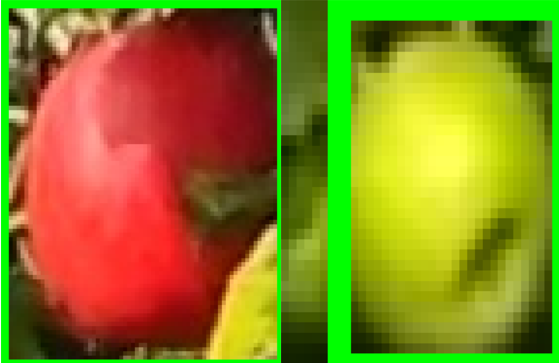
\includegraphics[width=0.3\textwidth]{images/contours_outcome.png}
    \caption{Two examples of the output for the counting test dataset by morphology and HSV based algorithm}
    \label{fig:output in the counting dataset}
\end{figure}

\subsubsection{Result in the detection dataset}
The examples of the output in the detection dataset by the morphology and HSV based algorithm are shown in Fig.~\ref{fig:output in the detection dataset}. Most of the pictures with clear red apples was detected in high precision and most of errors came from recognizing linked apples as a single one. For apples which are unclear and with various colours, the performance significantly decreased as it cannot recognize the fuzzy targets and misclassifies green objects in the background as green apples.

\begin{figure}[htb]
    \centering
    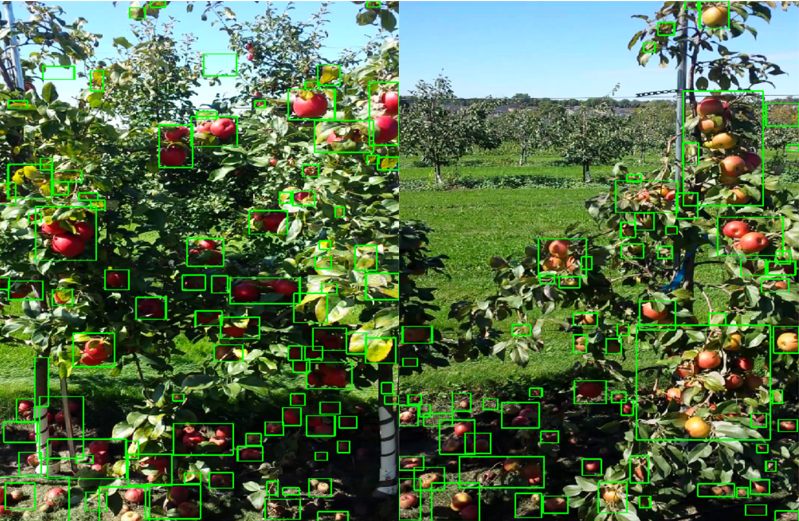
\includegraphics[width=0.75\textwidth]{images/result_mor_detect.png}
    \caption{Two examples of the output for the detection test dataset by morphology and HSV based algorithm}
    \label{fig:output in the detection dataset}
\end{figure}

\subsection{Results B——Deep Learning}
The results of the experiments on the counting test dataset and the detection test dataset by the deep learning method are summarised in Tab.~\ref{tab:results_YOLO}. It achieved 91.93\% and 84.80\% precision on the counting and detection test datasets in 2975 seconds and 1883 seconds respectively. As the task became more difficult, there was no significant drop in precision, while the running time was instead shortened by around 1,000 seconds.

\begin{table}[htb]
\centering
\caption{Results of the deep learning method}
\label{tab:results_YOLO}
\resizebox{\textwidth}{!}{%
\begin{tabular}{@{}p{5cm}<{\centering} p{5cm}<{\centering} p{5cm}<{\centering}@{}}
\toprule
Dataset   & Precision & Running time/s \\ \midrule
Counting  & 0.9193 & 2975       \\
Detection & 0.8480 & 1883      \\ \bottomrule
\end{tabular}%
}
\end{table}

\subsubsection{Result in the counting dataset}
The examples of the output in the counting dataset by the deep learning method are shown in Fig.~\ref{fig:result_count_YOLO}. Limited by the quality of the images, the correctness is high for single presence or single absence cases. However, for multiple targets, the deep learning method occasionally identifies multiple targets as one or none.

\begin{figure}[htb]
    \centering
    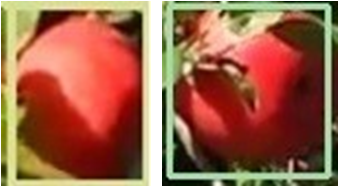
\includegraphics[width=0.4\textwidth]{images/result_YOLO_count.png}
    \caption{Two examples of the output for the counting test dataset by the deep learning method}
    \label{fig:result_count_YOLO}
\end{figure}

\subsubsection{Result in the detection dataset}
The examples of the output in the detection dataset by the deep learning method are shown in Fig.~\ref{fig:result_detect_YOLO}. For apples on trees and without occlusion, it makes an accurate detection, but for apples on the ground, it does not. At the same time, in environments with large light ratios, for instance, shadows deprive the apples of their colour information, leading to poor recognition. Nevertheless, for practical reasons, it is reasonable to record the number of apples on the tree. 

\begin{figure}[!ht]
    \centering
    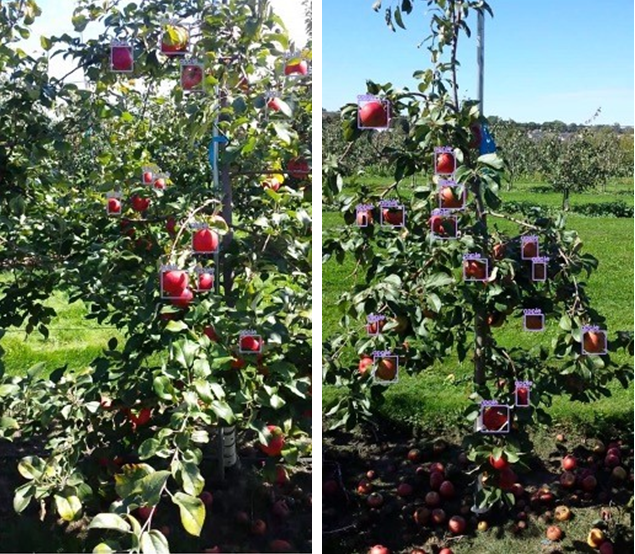
\includegraphics[width=0.6\textwidth]{images/result_YOLO_detect.png}
    \caption{Two examples of the output for the detection test dataset by the deep learning method}
    \label{fig:result_detect_YOLO}
\end{figure}


\subsection{Comparison}

\subsubsection{Running Time}
We tested both algorithms on the same platform, with the hardware parameters shown in Tab.~\ref{tab:Hardwares}. To be fair, we turned off the GPU acceleration and ran the performance on the CPU. The results are listed in Tab.~\ref{tab:running_time_test}.

We found that traditional image processing algorithms are able to complete the task quickly, whereas deep learning, due to its massive number of parameters, consumes more than a hundred times as much time. Furthermore, the number of images is another factor that affects YOLOX's performance, that is, YOLOX does not recognise a great number of small images as fast as it does a lesser number of large and complex images. 

\begin{table}[htb]
\centering
\caption{Results of the running time tests for the two algorithms}
\label{tab:running_time_test}
\resizebox{\textwidth}{!}{%
\begin{tabular}{@{}p{7cm}<{\centering} p{4cm}<{\centering} p{4cm}<{\centering}@{}}
\toprule
                                   & Counting dataset & Detection dataset \\ \midrule
Morphology and HSV based algorithm & 0.2272 s        & 12.6491 s         \\
YOLOX without GPU                              & 2975 s          & 1883 s            \\ \bottomrule
\end{tabular}%
}
\end{table}

Afterwards, we turned on GPU acceleration on a NVIDIA RTX2070 with $8\ GB$ of VRAM, and the running times were reduced to 187 and 156 seconds on the counting and detection datasets. But still a far cry from traditional image processing.

\subsubsection{Precision}
From Tab.~\ref{tab:results_morph} and Tab.~\ref{tab:results_morph}, the precision and average precision of YOLOX is significantly higher than that of the morphology and HSV based algorithm (26.03\% and 46.83\%), specifically in complex environments and with a significant number of targets. It should be noted that the precision of YOLOX does not decrease considerably as the complexity of the environment increases. In contrast, the precision of the morphology and HSV based algorithm decreased by up to 35\%. This indicates that deep learning models are more adaptable to complex tasks than traditional image processing. 

\subsubsection{Energy-precision Ratio}

As the robot needs to consider energy consumption when performing its tasks, we included the analysis of the energy-precision ratio because it reflects the difference in the precision of the models on the same energy consumption. The expression is:
\begin{equation}
    \left\{\begin{matrix}
    R = \frac{A}{W}  \\
    W = \sum p_h\times T
    \end{matrix}\right.
\end{equation}

where $W$ is the sum of the products of power and time ($T$) for all hardwares. The energy-precision ratios for the AMD 2600X and NVIDIA RTX2070 are 65 and 175 watts respectively, which gives the energy-precision ratios in Tab.~\ref{tab:energy-accuracy ratio test}. Morphology and HSV based algorithm has a much higher energy-precision ratio than deep learning, and the energy-precision ratio of YOLOX with GPU is lower than that of YOLOX without GPU. Morphology and HSV based algorithm therefore has an advantage in this indicator.

\begin{table}[htb]
\centering
\caption{The results of the energy-precision ratio test}
\label{tab:energy-accuracy ratio test}
\resizebox{\textwidth}{!}{%
\begin{tabular}{@{}p{7cm}<{\centering} p{4cm}<{\centering} p{4cm}<{\centering}@{}}
\toprule
                                   & Counting dataset       & Detection dataset      \\ \midrule
Morphology and HSV based algorithm & 0.04662                & 0.00046                \\
YOLOX with GPU                     & $4.7540\times 10^{-6}$ & $6.9284\times 10^{-6}$ \\
YOLOX without GPU                  & $2.0484\times 10^{-5}$ & $2.2650\times 10^{-5}$ \\ \bottomrule
\end{tabular}%
}
\end{table}

\subsubsection{Overall Analysis}
Considering running time, precision, and power consumption, we believe that both traditional and deep learning approaches are irreplaceable in terms of applications. Deep learning is more suitable for scenarios that require high precision and power consumption is not a concern. Traditional image processing is more suitable for simple and energy-limited environments. It should be noted that since the robot is in motion, the only deployment of CPU for deep learning may result in frame skipping, which leads to a reduction in real-time precision and affect the robot's judgement. As for energy-precision ratio, the savings in time costs by adding GPUs also compensates for power consumption with the help of proprietary components. 